\chapter{Locality-Awareness}
\label{chapter:Locality-aware}

\begin{figure*}[tb]
    \centering
    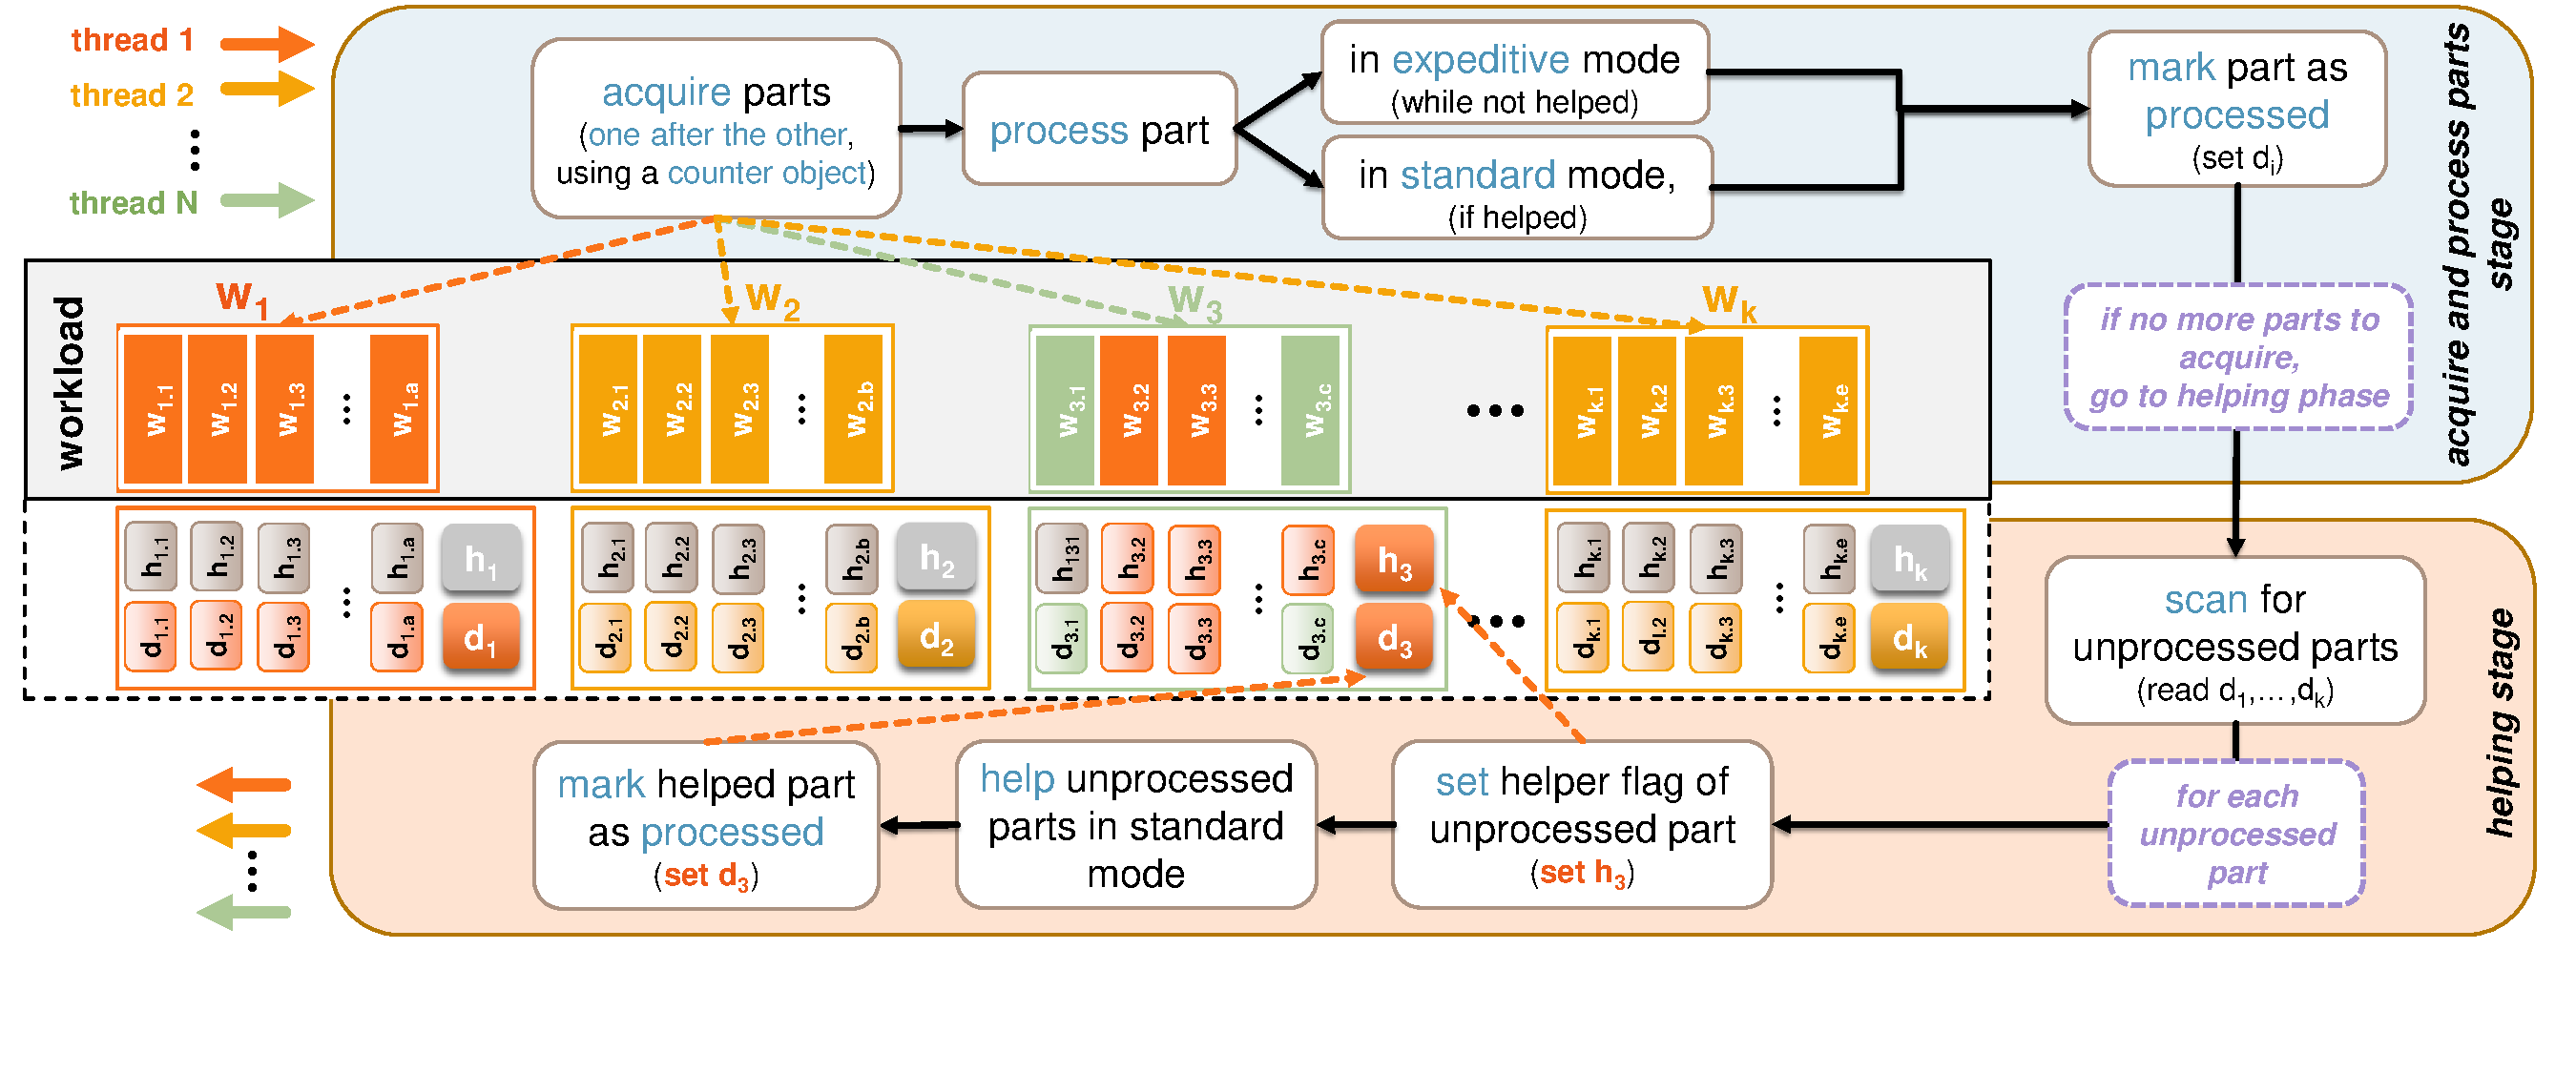
\includegraphics[width=\textheight,angle=90]{figures/locality-aware/Refresh_ekosmas_2-Themis.pdf}
    \caption{Refresh flowchart.}
	\label{fig:refresh:flowchart}
\end{figure*}

\section{Static iSAX-based Indexes}

{\em Locality-awareness}  aims at capturing several design principles (Definition~\ref{def:principles})
for data series indexes which are crucial for achieving good performance.
A locality aware implementation respects these principles. 
% 
\begin{definition}
\label{def:principles}
Principles for {\em locality-aware} processing:
\begin{enumerate}
\item \normalfont
{\bf Data Locality.} Separate the data into {\em disjoint sets} and have a distinct thread
processing the data of each set. This results in reduced communication 
cost (cache misses and branch misprediction) among the threads.
\item \normalfont
{\bf High Parallelism \& Low Synchronization Cost.} 
Threads should work in parallel and independently from each other as much as possible. 
Whenever synchronization cannot be avoided, design the appropriate 
mechanisms to minimize its cost.
\item \normalfont
{\bf Load Balancing.} Share the workload equally to the different threads, thus
avoiding load imbalances between threads and having all threads busy at each
point in time. 

\end{enumerate}
\end{definition}
% 
Enuring locality awareness results in good performance and is thus 
a desirable property for big data processing. In existing static  iSAX-based indexes, 
a thread operates on chunks of \textit{RawData} and processes disjoint sets of summarization
buffers and subtrees of the index tree. Also, an iSAX-based index employs 
several priority queues to store leaf nodes containing candidate series.
Thus, iSAX-based indexes are {\em locality-aware}.

To describe \textit{ReFreSh} in more detail, consider a {\em blocking} locality-aware
implementation $\mathcal{A}$, which splits its workload into disjoint parts and assigns them to 
threads for processing. 
% 
The main idea behind it is to require from each thread that completes processing
its own workload (instead of blocking, waiting for other threads to also finish) 
to scan for unprocessed workloads (e.g. in an iSAX-based index, unprocessed parts of $RawData$
or unprocessed summarization buffers), and help completing their processing. 

\textit{ReFreSh} (Algorithm~\ref{alg:refresh}) transforms $\mathcal{A}$ into a {\em lock-free} 
locality-aware implementation $\mathcal{B}$ that achieves high parallelism. 
% 
Let $W$ be the workload that $\mathcal{A}$ processes 
and let $w_1, \ldots, w_k$ be the parts it is separated to ensure locality awareness.
\textit{ReFreSh} applies for each data structure $D$ of $\mathcal{A}$, 
the following steps (depicted in Figure~\ref{fig:refresh:flowchart}):


%%%%%%%%%%%%%%%%%%%%%%%%%%%%%%% REFRESH ALGORITHM %%%%%%%%%%%%%%%%%%%%%%%%%%%%%%%%%%%%%% 

\begin{algorithm}[htbp]
    \footnotesize
    \vspace*{2mm}
    
    \begin{algorithmic}[1]
    
    \Procedure{InitializeSharedVariables}{}
        \State Workload part $\mathit{W} \gets [w_1, w_2, \ldots, w_k]$ \label{alg:refresh:w}
        \State Boolean array $\mathit{D} \gets [d_1, d_2, \ldots, d_k]$, initially $d_i = \False$ \label{alg:refresh:d}
        \State Boolean array $\mathit{H} \gets [h_1, h_2, \ldots, h_k]$, initially $h_i = \False$ \label{alg:refresh:h}
    \EndProcedure
    
    \vspace*{1mm}
    \State{Code for each thread:}    
    \vspace*{1mm}
    
    \Procedure{Refresh}{}
        \While{$\mathit{W}$ has available parts}  \label{alg:refresh:process:start}
            \State $\mathit{w_i} \gets$ Acquire an available part of $\mathit{W}$
            \State Mark $\mathit{w_i}$ as acquired
            \If{$h_i == \False$}  \label{alg:refresh:process:if}
                \State Process $\mathit{w_i}$ in expeditive mode, while checking that $h_i$ remains $\False$ \label{alg:refresh:process:expeditive}
                \State If $h_i == \True$, switch to standard mode
            \Else
                \State Process $\mathit{w_i}$ in standard mode \label{alg:refresh:process:standard}
            \EndIf
            \State $d_i \gets \True$ \label{alg:refresh:d:true}
        \EndWhile
        
        \vspace*{1mm}
        \ForAll{$d_i \in D$ where $d_i == \False$}  \label{alg:refresh:scan:ForAll} 
            \State Backoff()  \Comment{Avoid helping, if possible} \label{alg:refresh:help:backoff}
            \If{$d_i == \False$}  \label{alg:refresh:help:if}
                \State $h_i \gets \True$ \label{alg:refresh:h:true}
                \State Process $\mathit{w_i}$ in standard mode, checking periodically if $d_i$ remains $\False$ \label{alg:refresh:help:process}
                \State If $d_i == \True$, stop processing $\mathit{w_i}$
                \State $d_i \gets \True$ \label{alg:refresh:help:d:true}
            \EndIf
        \EndFor
    \EndProcedure
    
    \end{algorithmic}
    
    \caption{\textit{ReFreSh} - A general approach for transforming a blocking data structure $\mathit{D}$ into a lock-free one.}
    \label{alg:refresh}
\end{algorithm}

\newpage

\begin{enumerate}
    \item It attaches a {\em flag} $d_i$, $1 \leq i \leq k$, (initially \False)  
    with each $w_i$ to identify whether $w_i$'s processing is done.  
    As soon as a thread finishes processing $w_i$, it sets $d_i$ to \True\ (line~\ref{alg:refresh:d:true}).  

    \item Threads in $\mathcal{B}$ execute the same algorithm as in $\mathcal{A}$ to acquire parts of $W$ to process,  
    until all parts have been acquired (lines~\ref{alg:refresh:process:start}-\ref{alg:refresh:d:true}).  
    The thread that acquires a workload is its {\em owner}.  

    \item To achieve lock-freedom, every thread $t$, then, {\em scans} all the flags ($d_i$, $1 \leq i \leq k$)  
    to find those parts that are still unfinished (line~\ref{alg:refresh:scan:ForAll}).  

    \item Thread $t$ {\em helps} by processing, one after the other, each part found unfinished during scan.  
    For each part $w_i$, $1 \leq i \leq k$, that $t$ helps, it periodically checks $d_i$  
    to see whether other threads completed the processing of $w_i$. If this is so,  
    $t$ stops helping $w_i$ (line~\ref{alg:refresh:help:process}).  
    A thread that completes the processing of $w_i$ changes $d_i$ to \True\ (line~\ref{alg:refresh:help:d:true}).  

    \item Due to helping, every data structure $D$, employed in $\mathcal{A}$, may be  
    concurrently accessed by many threads. Thus, $\mathcal{B}$ should provide an efficient  
    lock-free implementation for all data structures of $\mathcal{A}$.  
\end{enumerate}


In locality-aware implementations threads are expected to work
on their own parts of the data most of the time ({\em contention-free phase}), and they
may help other threads only for a small period of time at the end of their execution
({\em concurrent phase}).
In the contention-free phase, \textit{ReFreSh} avoids synchronization overheads incurred to
ensure lock-freedom. 
Specifically, it employs two implementations for each data structure $D$ of  $\mathcal{A}$,
one with low synchronization cost that does not support helping ({\em expeditive mode}),
and another that supports helping and has higher synchronization overhead ({\em standard mode}).  
To enable threads operate on the appropriate mode,  a {\em helping-indicator flag} $h_i$ 
(initially \False) , $1 \leq i \leq k$, is attached with each $w_i$, which indicates whether 
$w_i$'s processing should be performed on expeditive or standard mode.
% 
A thread $t$ starts by processing its assigned workload 
on expeditive mode (lines~\ref{alg:refresh:h} and \ref{alg:refresh:process:if}-\ref{alg:refresh:process:expeditive}).
Before $t$ starts helping some part $w_i$, it sets $h_i$ to \True\ (line~\ref{alg:refresh:h:true}),
to alert $w_i$'s owner thread to start running on standard mode (line~\ref{alg:refresh:process:expeditive}).

To avoid helping whenever it is not absolutely necessary, i.e. when no thread has
failed (or is extremely slow), \textit{RefreSh} provides an optional {\em backoff scheme} that is used
by every thread $t$ (line~\ref{alg:refresh:help:backoff}) 
before it attempts to help other threads (line~\ref{alg:refresh:help:if}-\ref{alg:refresh:help:process}).
A small delay before switching to standard mode, often positively affects performance.
The delay is usually an estimate of the actual time a thread requires to finish its
current workload, calculated at run time.
% 
To minimize the work performed by a helper, \textit{ReFreSh} could
be applied  {\em recursively} by splitting each part $w_i$ to subparts. 
This way, a helper helps only the remaining unfinished subparts of $w_i$
and not the whole $w_i$. Thus, the redundant work is further decreased. 
To achieve this, the subparts of $w_i$ should have their own flag and helping-indicator variables.

Lock-freedom is ensured due to the {\em helping code} (lines~\ref{alg:refresh:scan:ForAll}-
\ref{alg:refresh:help:d:true}). In \textit{ReFreSh}, only after a thread
$t$ processes a workload $w_i$, it sets $h_i$ to \True\, and $t$ performs 
the helping code after finishing with its assigned workloads. Thus, when $t$ completes
its helping code the processing of all parts of the workload has been completed. 
This means that $t$ may continue directly to the execution of the next stage, without
waiting for the other threads to complete the execution of the current stage. 
Therefore, this scheme renders the use of barriers useless, as needed to achieve lock-freedom. 

Summarizing, \textit{ReFreSh} is a general scheme for processing a locality-aware
static workload in a lock-free way, without sacrificing locality-awareness. 


\subsection{\textbf{ReFreSh with Dynamic Batches}}  

In an iSAX-based index, \textit{ReFreSh} is applied to all stages to implement the traverse
method. When data arrives dynamically in batches, \textit{ReFreSh} must be applied to process
each batch. This brings some complications when processing data structures such as the summarization
buffers and the iSAX tree.
% 
The core issue lies in how \textit{ReFreSh} determines when to switch execution modes.
Its behavior relies on boolean flags that initially have the value \texttt{False} to 
indicate execution in expeditive mode and transition
to \texttt{True} when processing becomes standard. After creating the initial index, processing any
ongoing batch will encounter these flags already set to \texttt{True}, causing \textit{ReFreSh} to 
run in \textit{standard mode}. This is suboptimal because \textit{standard mode} enables helping,
which is unnecessary unless a helper has actually arrived. To avoid such uneccessary performance
penalties,\textit{ReFreSh} must be modified to support dynamic batch processing effectively.  

To continue ensuring locality-awareness each batch is processed in a locality-aware way. 
Specifically for each batch $b_j$, let $w_j$ be the workload for processing $b_j$ 
and let $w(j,i)$ $1 \leq i \leq k$, be the parts of this workload.
Thus, for each batch $b_j$ we define flags $d(j,i)$, $h(j,i)$ and we run an instance
of \Refresh. Moreover we apply the following modifications:

\begin{enumerate}  
    \item \textbf{Replacing Boolean Flags with Counters:}  
    Instead of using boolean flags, DFreSh replaces them with counters. Each part $w(j,i)$,
    is assigned a counter $d(j,i)$ (initially set to 0). This counter tracks whether $w(j,i)$ has
    completed processing part $w(j,i)$ for $b_j$. Once a thread finishes processing $w(j,i)$, it
    sets $d(j,i)$ to $\mathit{j} + 1$, which corresponds to the index of the next
    batch (see Algorithm~\ref{alg:DRefresh}).  

    \item \textbf{Batch-Aware Execution of \textit{ReFreSh}:}  
    Each time \textit{ReFreSh} is executed while processing batch $b_j$, the following holds:
    \begin{itemize}  
        \item A part $w(j,i)$ is considered processed for a batch with index $j$ when $d(j,i) = j + 1$.  
        \item A helper has arrived at part $w(j,i)$ for batch $b_j$ when $h(j,i) = j + 1$.  
    \end{itemize}  
\end{enumerate}  
% 
By implementing these modifications, we ensure that (a) execution mode transitions 
occur only when necessary and (b) \textit{ReFreSh} is correctly reused when moving 
from one batch to another.
These changes on Algorithm~\ref{alg:refresh} are illustrated with red in Algorithm~\ref{alg:DRefresh}.

%%%%%%%%%%%%%%%%%%%%%%%%%%%%%%% Dynamic Refresh %%%%%%%%%%%%%%%%%%%%%%%%%%%%%%%%%%%%%%%%

\begin{algorithm}[htbp]
    \footnotesize
    \vspace*{2mm}
    
    \begin{algorithmic}[1]
    
    \State \textbf{Shared variables:}
    \State Workload part $\mathit{W_j} := \mathit{[w(j,1), w(j,2), \ldots, w(j,k)]}$ \label{alg:DRefresh:w}
    \State \textbf{Int} array $\mathit{D_J} := \mathit{[d(j,1), d(j,2), \ldots, d(j,k)]}$, initially $\mathit{d(j,i)} = 0, \forall i \in {1,...,k}$ \label{alg:DRefresh:d}
    \State \textbf{Int} array $\mathit{H_J} := \mathit{[h(j,1), h(j,2), \ldots, h(j,k)]}$, initially $\mathit{h(j,i)} = 0, \forall i \in {1,...,k}$ \label{alg:DRefresh:h}
    
    \vspace*{1mm}
    \State \textbf{Code for each thread:}
    
    \Procedure{DRefresh}{int $\mathit{j}$}
        \While{$\mathit{W}$ has available parts} \label{alg:DRefresh:process:start}
            \State $\mathit{w(j,i)} \gets$ acquire an available part of $\mathit{W_j}$
            \State Mark $\mathit{w(j,i)}$ as acquired \label{alg:DFreSh:acquire-part}
            \If{\rb{$(\mathit{h(j,i)} == \mathit{j})$} \textbf{or} \rb{$(\mathit{d(j,i)} == \mathit{j}$ 
            \textbf{and} $\mathit{h(j,i)} < \mathit{j})$}} \label{alg:DRefresh:process:if}
                \State Process $\mathit{w(j,i)}$ in expeditive mode, while checking the value of $h(j,i) \leq j$ \label{alg:DRefresh:process:expeditive}
                \If{\rb{$\mathit{h(j,i)} == \mathit{j} + 1$}}\label{alg:DFreSh:switch-mode}
                    \State Switch to standard mode
                \EndIf
            \Else
                \State Process $\mathit{w(j,i)}$ in standard mode \label{alg:DRefresh:process:standard}
            \EndIf
            \State \rb{$\mathit{CAS(\&d(j,i), j, j+1)}$} \label{alg:DRefresh:d:increase}
        \EndWhile
        
        \ForAll{$\mathit{d(j,i)} \in D$ where $\mathit{d(j,i)} == \mathit{j}$} \label{alg:DRefresh:scan:ForAll} 
            \State Backoff() \label{alg:DRefresh:help:backoff}
            \rb{\If{$\mathit{d(j,i)} == \mathit{j}$} \label{alg:DRefresh:help:if}
                \If{$\mathit{h(j,i)} == \mathit{j}$} \label{alg:DRefresh:h:true}
                    \State $\mathit{CAS(\&h(j,i), j, j+1)}$ 
                \ElsIf{$\mathit{h(j,i)} < \mathit{j}$}      \label{alg:DRefresh:h:fallenBehind}
                    \State \textbf{int} oldVal $\gets \mathit{h(j,i)}$
                    \State $\mathit{CAS(\&h(j,i), oldVal, j+1)}$ \label{alg:DRefresh:h:CAS}
                \EndIf
            \EndIf
            }
            \State Process $\mathit{w(j,i)}$ in standard mode, checking $\mathit{d(j,i)} == j$
            \rb{\State $\mathit{CAS(\&d(j,i), j, j+1)}$ }\label{alg:DRefresh:help:d:true}
        \EndFor
    \EndProcedure
    
    \end{algorithmic}
    
    \caption{Dynamic version of ReFresh - Code for processing batch $B_j$.}
    \label{alg:DRefresh}
    \end{algorithm}

    We explain these changes in more detail below.

    \begin{enumerate}
        \item As in \textit{ReFreSh}, threads acquire parts (line~\ref{alg:DFreSh:acquire-part}) of the
        workload $W_j$ of batch $B_j$ for processing until all parts have been acquired. Each thread
        must determine the appropriate processing mode (lines~\ref{alg:DRefresh:process:if}-
        \ref{alg:DRefresh:process:standard}). A helper has arrived at part $w(j,i)$ of
        batch $B_j$ if the value of $h(j,i)$ is equal to $j + 1$ (line~\ref{alg:DFreSh:switch-mode}).
        Similarly a part $W(j,i)$ is considered processed if the value of $d(j,i)$ is equal to $j+1$.
        Once a thread finishes processing a part, it must try to atomically increment $d(j,i)$ using a
        compare-and-swap (CAS) operation to ensure correctness, as multiple threads may attempt
        to update it simultaneously (line~\ref{alg:DRefresh:d:increase}). 
        We apply an optimization to reduce the number of failed executed compare-and-swap (CAS)
        instructions by checking whether its value is already greater than $j$ which is the old value
        before performing the actual compare-and-swap
        (this optimization is not visible in Algorithm~\ref{alg:DRefresh} for simplicity)

    
        \item To maintain lock-freedom, after all parts become acquired every thread $t$ 
        has to check for unfinished parts in case some threads become slow
        (lines~\ref{alg:DRefresh:scan:ForAll}-\ref{alg:DRefresh:help:d:true}). A part 
        $w(j,i)$ is considered unprocessed if the value of $d(j,1)$ is equal to $j$.
          
        \item While processing unfinished parts of batch $b_j$ thread $t$ periodically checks $d(j,i)$  
        to determine whether other threads have already completed the processing of part $w(j,i)$.
        For each unfinished part $w(j,i)$ that thread $t$ encounters, it first attempts to inform other
        threads, which may be working on the same part, that multiple threads are now processing it
        concurrently. To better understand the pseudocode, let's focus on a specific $i$ and analyze
        what happens with helpers on the $i_{th}$ part of each batch. If during the processing of the
        previous batch a helping thread existed for part $w(j,i)$, then the if condition
        on line~\ref{alg:DRefresh:h:true} is executed. Otherwise, if there was no helper because that
        part was already processed during the scan (lines~\ref{alg:DRefresh:scan:ForAll}-\ref{alg:DRefresh:help:if})
        the else if condition on line (line~\ref{alg:DRefresh:h:fallenBehind}) is executed. 
        The compare-and-swap (CAS) has to figure out the correct old value to use in order to update
        the value of the flag (line~\ref{alg:DRefresh:h:CAS}).
    \end{enumerate}

The flowchart of how \Refresh\ works is shown in Figure~\ref{fig:refresh:flowchart} where 
all the described above mechanisms are visible for a batch $b_j$.